\subsection{1.1 Математическая модель и постановка задач}
Рассмотрим систему массового обслуживания $M|H_2|2$ с обратной связью (Рисунок \ref{fig:system2}).
\begin{figure}[htbp]
	\centering
	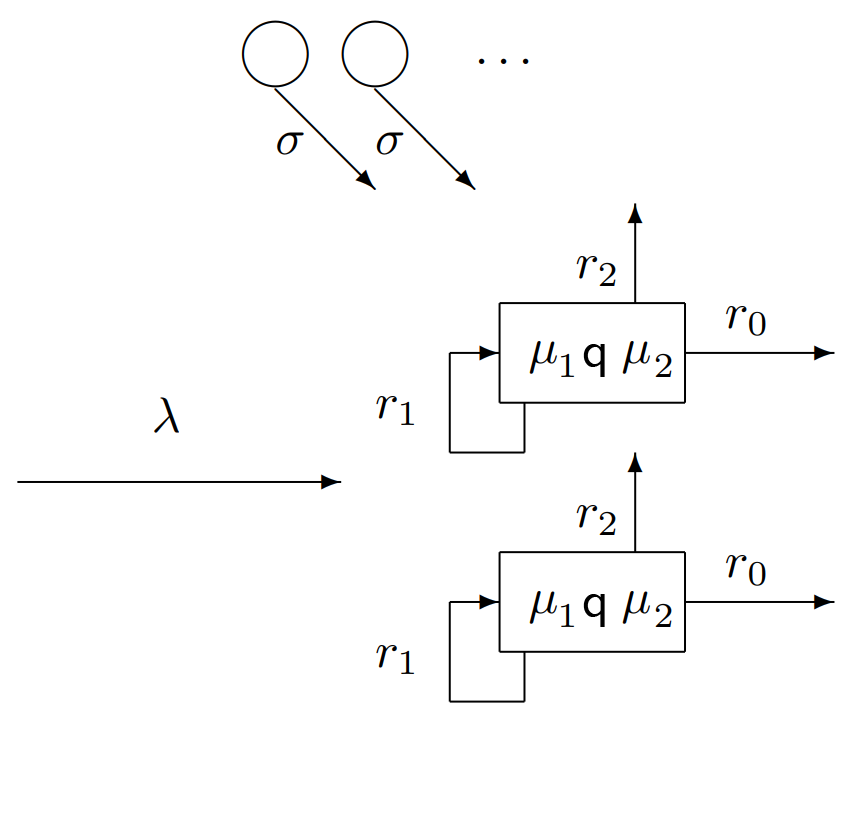
\includegraphics[width=0.5\textwidth]{system2}
	\caption{Система массового обслуживания M|$H_{2}$|2 с обратной связью}
	\label{fig:system2}
\end{figure}


Система имеет два обслуживающих прибора. Заявки поступают в систему согласно простейщиму потоку с параметром $\lambda$. Каждая заявка занимеет один из свободных приборов на время, распределенное по гиперэкспоненциальному закону. Это означает, что заявка на приборе с вероятностью $q$ поступает на первую фазу, с экспоненциальным распределением с параметром $\mu_{1}$, и с вероятность $1-q$ на вторую, с параметром $\mu_{2}$.

После завершения обслуживания заявка с вероятностью $r_{0}$ покидает систему, с вероятностью $r_{1}$ мгновенно поступает на повторное обслуживание и с вероятностью $r_{2}$ уходит на орбиту. Также, если на момент поступления заявки из потока оба прибора заняты, то заявка уходит на орбиту. Через время, продолжительность которого распределена по экспоненциальному закону с пареметром $\sigma$, заявка вновь обращается с орбиты к приборам.

Пусть $i(t)$ -- число заявок на орбите в момент времени $t$, 
$n_{1}(t)$ -- число приборов занятых на первой фазе в момент времени $t$,
$n_{2}(t)$ -- число приборов занятых на второй фазе в момент времени $t$.

Рассмотрим трехмерный процесс $\{n_{1}(t), n_{2}(t), i(t)\}$. Под состоянием системы будем понимать состояние процесса $\{n_{1}(t), n_{2}(t), i(t)\}$ в момент времени $t$.

Обозначим вероятности следующим образом:\\
$P(n_{1}=0,n_{2}=0,i(t)=i)=P_{0}(i, t)$ -- вероятность того, что ни один прибор не занят.\\
$P(n_{1}=0,n_{2}=1,i(t)=i)=P_{1}(i, t)$ -- вероятность того, что один прибор занят на второй фазе.\\
$P(n_{1}=1,n_{2}=0,i(t)=i)=P_{2}(i, t)$ -- вероятность того, что один прибор занят на первой фазе.\\
$P(n_{1}=0,n_{2}=2,i(t)=i)=P_{3}(i, t)$ -- вероятность того, что два прибора заняты на второй фазе.\\
$P(n_{1}=1,n_{2}=1,i(t)=i)=P_{4}(i, t)$ -- вероятность того, что один прибор занят на первой фазе, а другой на второй.\\
$P(n_{1}=2,n_{2}=0,i(t)=i)=P_{5}(i, t)$ -- вероятность того, что два прибора заняты на первой фазе.\\
В каждой вероятности на орбите находятся $i$ заявок в момент времени $t$.

Для решения будем применять методы асимптотического анализа [1, 7, 9, 11] и асимптотически диффузионного анализа [1].

\newpage

\subsection{1.2 Уравнения Колмогорова}


Для введенных вероятностей составим систему уравнений в конечных разностях [4, 5, 6]. 
\begin{adjustwidth}{0pt}{0pt}
	\begin{align*} 
		P_{0}(i,t+\Delta t)=&(1-\Delta t(\lambda+i\sigma))P_{0}(i,t)+\Delta t\mu_{2}r_{0}P_{1}(i,t)+\Delta t\mu_{2}r_{2}P_{1}(i-1,t)+\\
		&{}+\Delta t\mu_{1}r_{0}P_{2}(i,t)+
		+\Delta t\mu_{1}r_{2}P_{2}(i-1,t)+o(\Delta t),\\
		P_{1}(i,t+\Delta t)=&(1-\Delta t(\lambda+i\sigma+\mu_{2}))P_{1}(i,t)+\Delta t\lambda(1-q)P_{0}(i,t)+\\
		&{}+\Delta t\sigma(i+1)(1-q)P_{0}(i+1,t)+2\Delta t\mu_{2}r_{0}P_{3}(i,t) + \mu_{2}r_{1}(1-q)P_{1}(i,t)+\\
		&{}+2\mu_{2}r_{2}P_{3}(i-1,t)+\Delta t\mu_{1}r_{0}P_{4}(i,t)+
		\Delta t\mu_{1}r_{2}P_{4}(i-1,t)+\\
		&{}+\Delta t\mu_{1}r_{1}(1-q)P_{2}(i,t)+o(\Delta t),\\
		P_{2}(i,t+\Delta t)=&(1-\Delta t(\lambda+i\sigma+\mu_{1}))P_{2}(i,t)+\Delta tq\lambda P_{0}(i,t)+\\
		&\Delta t\sigma(i+1)qP_{0}(i+1,t)+\Delta t\mu_{2}r_{1}qP_{1}(i,t)+\\
		&+\Delta t\mu_{1}r_{1}qP_{2}(i,t)+\Delta t\mu_{2}r_{0}P_{4}(i,t)+\Delta t\mu_{2}r_{2}P_{4}(i-1,t)+\\
		&+2\Delta t\mu_{1}r_{2}P_{5}(i-1,t)+2\Delta t\mu_{1}r_{0}P_{5}(i,t)+o(\Delta t),\\
		P_{3}(i,t+\Delta t)=&(1-\Delta t(\lambda+i\sigma+2\mu_{2}))P_{3}(i,t)+\\
		&+\Delta t\lambda(1-q)P_{1}(i,t)+\Delta t\sigma(i+1)(1-q)P_{1}(i+1,t)+\\
		&+2\Delta t\mu_{2}r_{1}(1-q)P_{3}(i,t)+\Delta t\mu_{1}r_{1}(1-q)P_{4}(i,t)+\Delta t\lambda P_{3}(i-1,t)+o(\Delta t),\\
		P_{4}(i,t+\Delta t)=&(1-\Delta t(\lambda+i\sigma+\mu_{1}+\mu_{2}))P_{4}(i,t)+\Delta t\lambda qP_{1}(i,t)+\Delta t\sigma(i+1)qP_{1}(i+1,t)+\\
		&+2\Delta t\mu_{2}r_{1}qP_{3}(i,t)+\Delta t\lambda(1-q)P_{2}(i,t)+\Delta t\sigma(i+1)(1-q)P_{2}(i+1,t)+\\
		&+\Delta t\mu_{2}r_{1}(1-q)P_{4}(i,t)+\Delta t\mu_{1}r_{1}qP_{4}(i,t)+\\
		&+2\Delta t\mu_{1}r_{1}(1-q)P_{5}(i,t)+\Delta t\lambda P_{4}(i-1,t)+o(\Delta t),\\
		P_{5}(i,t+\Delta t)=&(1-\Delta t(\lambda+i\sigma+2\mu_{1}))P_{5}(i,t)+\Delta t\sigma(i+1)qP_{2}(i+1,t)+\Delta t\lambda qP_{2}(i,t)+\\
		&+\Delta t\mu_{2}r_{1}qP_{4}(i,t)+2\Delta t\mu_{1}r_{1}qP_{5}(i,t)+\Delta t\lambda P_{5}(i-1,t)+o(\Delta t).
	\end{align*}
\end{adjustwidth}
Расскроем скобки, разделим на каждое уравнение на $\Delta t$, получим
\begin{adjustwidth}{0pt}{0pt}
	\begin{align*} 
		\frac{P_{0}(i,t+\Delta t) - P_{0}(i, t)}{\Delta t}=&-(\lambda+i\sigma)P_{0}(i,t)+\mu_{2}r_{0}P_{1}(i,t)+\mu_{2}r_{2}P_{1}(i-1,t)+\mu_{1}r_{0}P_{2}(i,t)+\\
		&{}+\mu_{1}r_{2}P_{2}(i-1,t),\\
		\frac{P_{1}(i,t+\Delta t) - P_{1}(i, t)}{\Delta t}=&-(\lambda+i\sigma+\mu_{2})P_{1}(i,t)+\lambda(1-q)P_{0}(i,t)+\sigma(i+1)(1-q)P_{0}(i+1,t)+\\
		&{}+2\mu_{2}r_{0}P_{3}(i,t) + \mu_{2}r_{1}(1-q)P_{1}(i,t)+2\mu_{2}r_{2}P_{3}(i-1,t)+\mu_{1}r_{0}P_{4}(i,t)+\\
		&{}+\mu_{1}r_{2}P_{4}(i-1,t)+\mu_{1}r_{1}(1-q)P_{2}(i,t),\\
	\end{align*}
\end{adjustwidth}

\begin{adjustwidth}{0pt}{0pt}
	\begin{align*}
		\frac{P_{2}(i,t+\Delta t) - P_{2}(i, t)}{\Delta t}=&-(\lambda+i\sigma+\mu_{1})P_{2}(i,t)+q\lambda P_{0}(i,t)\\
		&+\sigma(i+1)qP_{0}(i+1,t)+\mu_{2}r_{1}qP_{1}(i,t)+\\
		&+\mu_{1}r_{1}qP_{2}(i,t)+\mu_{2}r_{0}P_{4}(i,t)+\mu_{2}r_{2}P_{4}(i-1,t)+\\
		&+2\mu_{1}r_{2}P_{5}(i-1,t)+2\mu_{1}r_{0}P_{5}(i,t),\\
		\frac{P_{3}(i,t+\Delta t) - P_{3}(i, t)}{\Delta t}=&-(\lambda+i\sigma+2\mu_{2})P_{3}(i,t)+\lambda(1-q)P_{1}(i,t)+\\
		&+\sigma(i+1)(1-q)P_{1}(i+1,t)+2\mu_{2}r_{1}(1-q)P_{3}(i,t)+\\
		&+\mu_{1}r_{1}(1-q)P_{4}(i,t)\lambda P_{3}(i-1,t),\\
		\frac{P_{4}(i,t+\Delta t) - P_{4}(i, t)}{\Delta t}=&-(\lambda+i\sigma+\mu_{1}+\mu_{2})P_{4}(i,t)+\lambda qP_{1}(i,t)+\sigma(i+1)qP_{1}(i+1,t)+\\
		&+2\mu_{2}r_{1}qP_{3}(i,t)+\lambda(1-q)P_{2}(i,t)+\sigma(i+1)(1-q)P_{2}(i+1,t)+\\
		&+\mu_{2}r_{1}(1-q)P_{4}(i,t)+\mu_{1}r_{1}qP_{4}(i,t)+2\mu_{1}r_{1}(1-q)P_{5}(i,t)+\\
		&+\lambda P_{4}(i-1,t),\\
		\frac{P_{5}(i,t+\Delta t) - P_{5}(i, t)}{\Delta t}=&-(\lambda+i\sigma+2\mu_{1})P_{5}(i,t)+\sigma(i+1)qP_{2}(i+1,t)+\lambda qP_{2}(i,t)+\\
		&+\mu_{2}r_{1}qP_{4}(i,t)+2\mu_{1}r_{1}qP_{5}(i,t)+\lambda P_{5}(i-1,t).
	\end{align*}
\end{adjustwidth}
Устремим $\Delta t \rightarrow 0$, получим 
\begin{align*} 
	\frac{dP_{0}(i,t)}{\partial t}=&-(\lambda+i\sigma)P_{0}(i,t)+\mu_{2}r_{0}P_{1}(i,t)+\mu_{2}r_{2}P_{1}(i-1,t)+\mu_{1}r_{0}P_{2}(i,t)+\\
	&{}+\mu_{1}r_{2}P_{2}(i-1,t),\\
	\frac{dP_{1}(i,t)}{\partial t}=&-(\lambda+i\sigma+\mu_{2})P_{1}(i,t)+\lambda(1-q)P_{0}(i,t)+\sigma(i+1)(1-q)P_{0}(i+1,t)+\\
	&{}+2\mu_{2}r_{0}P_{3}(i,t) + \mu_{2}r_{1}(1-q)P_{1}(i,t)+2\mu_{2}r_{2}P_{3}(i-1,t)+\mu_{1}r_{0}P_{4}(i,t)+\\
	&{}+\mu_{1}r_{2}P_{4}(i-1,t)+\mu_{1}r_{1}(1-q)P_{2}(i,t),\\
	\frac{dP_{2}(i,t)}{\partial t}=&-(\lambda+i\sigma+\mu_{1})P_{2}(i,t)+q\lambda P_{0}(i,t)+\sigma(i+1)qP_{0}(i+1,t)+\mu_{2}r_{1}qP_{1}(i,t)+\\
	&+\mu_{1}r_{1}qP_{2}(i,t)+\mu_{2}r_{0}P_{4}(i,t)+\mu_{2}r_{2}P_{4}(i-1,t)+2\mu_{1}r_{2}P_{5}(i-1,t)+\\
	&+2\mu_{1}r_{0}P_{5}(i,t),\\
	\frac{dP_{3}(i,t)}{\partial t}=&-(\lambda+i\sigma+2\mu_{2})P_{3}(i,t)+\lambda(1-q)P_{1}(i,t)+\sigma(i+1)(1-q)P_{1}(i+1,t)+\\
	&+2\mu_{2}r_{1}(1-q)P_{3}(i,t)+\mu_{1}r_{1}(1-q)P_{4}(i,t)+\lambda P_{3}(i-1,t),\\
	\frac{dP_{4}(i,t)}{\partial t}=&-(\lambda+i\sigma+\mu_{1}+\mu_{2})P_{4}(i,t)+\lambda qP_{1}(i,t)+\sigma(i+1)qP_{1}(i+1,t)+\\
	&+2\mu_{2}r_{1}qP_{3}(i,t)+\lambda(1-q)P_{2}(i,t)+\sigma(i+1)(1-q)P_{2}(i+1,t)+\\
	&+\mu_{2}r_{1}(1-q)P_{4}(i,t)+\mu_{1}r_{1}qP_{4}(i,t)+2\mu_{1}r_{1}(1-q)P_{5}(i,t)+\lambda P_{4}(i-1,t),\\
	\frac{dP_{5}(i,t)}{\partial t}=&-(\lambda+i\sigma+2\mu_{1})P_{5}(i,t)+\sigma(i+1)qP_{2}(i+1,t)+\lambda qP_{2}(i,t)+\\
	&+\mu_{2}r_{1}qP_{4}(i,t)+2\mu_{1}r_{1}qP_{5}(i,t)+\lambda P_{5}(i-1,t).
\end{align*} 
Введем частичные характерестические функции
$$H_{k}(u,t)=\sum_{i=0}^\infty e^{iuj}P_{k}(i,t).$$
Тогда система примет вид
\begin{align*} 
	\frac{dH_{0}(u,t)}{\partial t}=&-\lambda H_{0}(u,t)+j\sigma \frac{dH_{0}(u,t)}{\partial u}+\mu_{2}r_{0}H_{1}(u,t)+\mu_{2}r_{2}e^{ju}H_{1}(u,t)+\\
	&+\mu_{1}r_{0}H_{2}(u,t)+\mu_{1}r_{1}e^{ju}H_{2}(u,t),\\
	\frac{dH_{1}(u,t)}{\partial t}=&-(\lambda+\mu_{2}) H_{1}(u,t)+j\sigma \frac{dH_{1}(u,t)}{\partial u}+\lambda(1-q)H_{0}(u,t)-\\
	&-j\sigma e^{-ju}(1-q) \frac{dH_{0}(u,t)}{\partial u}+2\mu_{2}r_{0}H_{3}(u,t)+\mu_{2}r_{1}(1-q)H_{1}(u,t)+\\
	&+2\mu_{2}r_{2}e^{ju}H_{3}(u,t)+\mu_{1}r_{0}H_{4}(u,t)+\mu_{1}r_{2}e^{ju}H_{4}(u,t)+\\
	&+\mu_{1}r_{1}(1-q)H_{2}(u,t),\\
	\frac{dH_{2}(u,t)}{\partial t}=&-(\lambda+\mu_{1}) H_{2}(u,t)+j\sigma \frac{dH_{2}(u,t)}{\partial u}+q\lambda  H_{2}(u,t)-j\sigma e^{-ju}q \frac{dH_{0}(u,t)}{\partial u}+\\
	&+\mu_{2}r_{1}qH_{1}(u,t)+\mu_{1}r_{1}qH_{2}(u,t)+\mu_{2}r_{0}H_{4}(u,t)+\mu_{2}r_{2}e^{ju}H_{4}(u,t)+\\
	&+2\mu_{1}r_{2}e^{ju}H_{5}(u,t)+2\mu_{1}r_{0}H_{5}(u,t),\\
	\frac{dH_{3}(u,t)}{\partial t}=&-(\lambda+2\mu_{2}) H_{3}(u,t)+j\sigma \frac{dH_{3}(u,t)}{\partial u}+\lambda(1-q) H_{1}(u,t)-\\
	&-j\sigma (1-q)e^{-ju} \frac{dH_{0}(u,t)}{\partial u}+2\mu_{2}r_{1}(1-q) H_{3}(u,t)+\\
	&+\mu_{1}r_{1}(1-q) H_{4}(u,t)+\lambda e^{ju} H_{3}(u,t),\\
	\frac{dH_{4}(u,t)}{\partial t}=&-(\lambda+\mu_{1}+\mu_{2}) H_{4}(u,t)+j\sigma \frac{dH_{4}(u,t)}{\partial u}+\lambda qH_{4}(u,t)-\\
	&-j\sigma qe^{-ju} \frac{dH_{1}(u,t)}{\partial u}+2\mu_{2}r_{1}qH_{3}(u,t)+\lambda(1-q)H_{2}(u,t)-\\
	&-j\sigma (1-q)e^{-ju} \frac{dH_{0}(u,t)}{\partial u}+\mu_{2}r_{1}(1-q)H_{4}(u,t)+\mu_{1}r_{1}qH_{4}(u,t)+\\
	&+2\mu_{1}r_{1}(1-q)H_{5}(u,t)+\lambda e^{ju}H_{4}(u,t),\\
	\frac{dH_{5}(u,t)}{\partial t}=&-(\lambda+2\mu_{1}) H_{5}(u,t)+j\sigma \frac{dH_{5}(u,t)}{\partial u}-j\sigma qe^{-ju} \frac{dH_{2}(u,t)}{\partial u}+\\
	&+\lambda qH_{2}(u,t)+\mu_{2}r_{1}qH_{4}(u,t)+2\mu_{1}r_{1}qH_{5}(u,t)+\lambda e^{ju}H_{5}(u,t).\\
\end{align*} 
Обозначим вектор-строки
\begin{align*}
	\boldsymbol{H}(u,t)=&\{H_{0}(u,t),H_{1}(u,t),H_{2}(u,t),H_{3}(u,t),H_{4}(u,t),H_{5}(u,t)\},\\
	\frac{\partial \boldsymbol{H}(u,t)}{\partial t}=&\{\frac{\partial H_{0}(u,t)}{\partial t},\frac{\partial H_{1}(u,t)}{\partial t},\frac{\partial H_{2}(u,t)}{\partial t},\frac{\partial H_{3}(u,t)}{\partial t},\frac{\partial H_{4}(u,t)}{\partial t},\frac{\partial H_{5}(u,t)}{\partial t}\},\\
	\frac{\partial \boldsymbol{H}(u,t)}{\partial u}=&\{\frac{\partial H_{0}(u,t)}{\partial u},\frac{\partial H_{1}(u,t)}{\partial u},\frac{\partial H_{2}(u,t)}{\partial u},\frac{\partial H_{3}(u,t)}{\partial u},\frac{\partial H_{4}(u,t)}{\partial u},\frac{\partial H_{5}(u,t)}{\partial u}\}.\\
\end{align*} 
Запишем систему уравнений в виде матричного уравнения
\begin{align*}
	\frac{\partial \boldsymbol{H}(u,t)}{\partial t}=\boldsymbol{H}(u,t)(\boldsymbol{A}+e^{ju}\boldsymbol{B})+j\sigma\frac{\partial \boldsymbol{H}(u,t)}{\partial u}(\boldsymbol{I_{0}}-e^{-ju}\boldsymbol{I_{1}}),
\end{align*} 
где
\begin{gather*} 
	\boldsymbol{A} =
	\!\begin{aligned}
		&
		\left[\begin{matrix}- \lambda & \lambda \left(1 - q\right) & \lambda q & 0% & 0 & 0
			\\r_{0} \mu_{2} & - \lambda + r_{1} \mu_{2} \left(1 - q\right) - \mu_{2} & q r_{1} \mu_{2} & \lambda \left(1 - q\right) %& \lambda q & 0
			\\r_{0} \mu_{1} & r_{1} \mu_{1} \left(1 - q\right) & - \lambda + q r_{1} \mu_{1} - \mu_{1} & 0% & \lambda \left(1 - q\right) & \lambda q
			\\0 & 2 r_{0} \mu_{2} & 0 & - \lambda + 2 r_{1} \mu_{2} \left(1 - q\right) - 2 \mu_{2} %& 2 q r_{1} \mu_{2} & 0
			\\0 & r_{0} \mu_{1} & r_{0} \mu_{2} & r_{1} \mu_{1} \left(1 - q\right) %& - \lambda + q r_{1} \mu_{1} + r_{1} \mu_{2} \left(1 - q\right) - \mu_{1} - \mu_{2} & q r_{1} \mu_{2}
			\\0 & 0 & 2 r_{0} \mu_{1} & 0 %& 2 r_{1} \mu_{1} \left(1 - q\right) & - \lambda + 2 q r_{1} \mu_{1} - 2 \mu_{1}
		\end{matrix}\right.\\
		&\qquad\qquad
		\left.\begin{matrix}
			{}0 & 0
			\\ {}\lambda q & 0
			\\ {}\lambda \left(1 - q\right) & \lambda q
			\\ {}2 q r_{1} \mu_{2} & 0
			\\ {}- \lambda + q r_{1} \mu_{1} + r_{1} \mu_{2} \left(1 - q\right) - \mu_{1} - \mu_{2} & q r_{1} \mu_{2}
			\\ {}2 r_{1} \mu_{1} \left(1 - q\right) & - \lambda + 2 q r_{1} \mu_{1} - 2
		\end{matrix}\right],
	\end{aligned}
\end{gather*}

\begin{gather*}
	\boldsymbol{B}=
	\!\begin{aligned}
		&
		\left[\begin{matrix}0 & 0 & 0 & 0 & 0 & 0\\\mu_{2} \left(- r_{0} - r_{1} + 1\right) & 0 & 0 & 0 & 0 & 0\\\mu_{1} \left(- r_{0} - r_{1} + 1\right) & 0 & 0 & 0 & 0 & 0\\0 & 2 \mu_{2} \left(- r_{0} - r_{1} + 1\right) & 0 & \lambda & 0 & 0\\0 & \mu_{1} \left(- r_{0} - r_{1} + 1\right) & \mu_{2} \left(- r_{0} - r_{1} + 1\right) & 0 & \lambda & 0\\0 & 0 & 2 \mu_{1} \left(- r_{0} - r_{1} + 1\right) & 0 & 0 & \lambda\end{matrix}\right],
	\end{aligned}
\end{gather*}

\begin{gather*}
	\boldsymbol{I_{0}}=
	\!\begin{aligned}
		&
		\left[\begin{matrix}1 & 0 & 0 & 0 & 0 & 0\\0 & 1 & 0 & 0 & 0 & 0\\0 & 0 & 1 & 0 & 0 & 0\\0 & 0 & 0 & 0 & 0 & 0\\0 & 0 & 0 & 0 & 0 & 0\\0 & 0 & 0 & 0 & 0 & 0\end{matrix}\right],
		&
		\boldsymbol{I_{1}}=
		&
		\left[\begin{matrix}0 & 1 - q & q & 0 & 0 & 0\\0 & 0 & 0 & 1 - q & q & 0\\0 & 0 & 0 & 0 & 1 - q & q\\0 & 0 & 0 & 0 & 0 & 0\\0 & 0 & 0 & 0 & 0 & 0\\0 & 0 & 0 & 0 & 0 & 0\end{matrix}\right].
	\end{aligned}
\end{gather*}
Домножим матричное уравнение на единичный вектор-столбец $\boldsymbol{e}$ и, с учетом $$(\boldsymbol{A} + \boldsymbol{B}) \boldsymbol{e} = 0$$ и $$(\boldsymbol{I_{0}} - \boldsymbol{I_{1}}) \boldsymbol{e} = 0$$ получим
\begin{align*}
	\frac{\partial \boldsymbol{H}(u,t)}{\partial t}\boldsymbol{e}=&\boldsymbol{H}(u,t)(e^{ju}-1)\boldsymbol{B}\boldsymbol{e}+j\sigma e^{-ju}\frac{\partial \boldsymbol{H}(u,t)}{\partial u}(e^{ju}-1)\boldsymbol{I_{0}}\boldsymbol{e}=\\
	&=(e^{ju}-1)\{\boldsymbol{H}(u,t)\boldsymbol{B}\boldsymbol{e}+j\sigma e^{-ju}\frac{\partial \boldsymbol{H}(u,t)}{\partial u}\boldsymbol{I_{0}} \boldsymbol{e}\}.
\end{align*} 
Таким образом получаем уравнения
\begin{equation}
	\begin{split}
		&\frac{\partial \boldsymbol{H}(u,t)}{\partial t}=\boldsymbol{H}(u,t)(\boldsymbol{A}+e^{ju}\boldsymbol{B})+j\sigma\frac{\partial \boldsymbol{H}(u,t)}{\partial u}(\boldsymbol{I_{0}}-e^{-ju}\boldsymbol{I_{1}}),\\
		&\frac{\partial \boldsymbol{H}(u,t)}{\partial t} \boldsymbol{e}=(e^{ju}-1)\{\boldsymbol{H}(u,t)\boldsymbol{B} \boldsymbol{e}+j\sigma e^{-ju}\frac{\partial \boldsymbol{H}(u,t)}{\partial u}\boldsymbol{I_{0}} \boldsymbol{e}\}.
	\end{split}
\end{equation}
\newpage
\subsection{1.3 Первый этап асимптотического анализа}

Будем решать уравнения (1) методом асимптотического анализа.
Сделаем замены
\begin{align}
	\sigma=\varepsilon ,\tau=t\varepsilon, u=\varepsilon w, \boldsymbol{H}(u,t)=\boldsymbol{F}(w,\tau, \varepsilon).
\end{align} 
Тогда можем переписать уравнения (1)
\begin{equation}
	\begin{split}
		&\varepsilon\frac{\partial \boldsymbol{F}(w,\tau,\varepsilon)}{\partial \tau} =\boldsymbol{F}(w,\tau,\varepsilon)(\boldsymbol{A}+e^{j\varepsilon w}\boldsymbol{B})+j\frac{\partial \boldsymbol{F}(w,\tau,\varepsilon)}{\partial w}(\boldsymbol{I_{0}}-e^{-j\varepsilon w}\boldsymbol{I_{1}}),\\
		&\varepsilon\frac{\partial \boldsymbol{F}(w,\tau,\varepsilon)}{\partial \tau}\boldsymbol{e} =(e^{j\varepsilon w}-1)\{\boldsymbol{F}(w,\tau,\varepsilon)\boldsymbol{B}\boldsymbol{e}+j e^{-j\varepsilon w}\frac{\partial \boldsymbol{F}(w,\tau,\varepsilon)}{\partial w}\boldsymbol{I_{0}}\boldsymbol{e}\}.
	\end{split}
\end{equation}
При условии, что $\varepsilon\rightarrow 0$, можно доказать следующее утверждение.\\

\textbf{Теорема 1.1.} Компоненты $R_{n}$ или вектор-строка R распределения вероятностей числа приборов, занятых на первой и второй фазе имеет вид
\begin{equation}
	\begin{split}
		&R_{0} = \frac{2 \mu_{1}^{2} \mu_{2}^{2} (r_{1} - 1)^{2}}{c},\\
		&R_{1} = \frac{2 \mu_{1}^{2} \mu_{2} (1 - q) (1 - r_{1})(\lambda + x)}{c},\\
		&R_{2} = \frac{2 \mu_{1} \mu_{2}^{2} q (1 - r_{1})(\lambda + x)}{c},\\
		&R_{3} = \frac{\mu_{1}^{2} (1 - q)^{2}(\lambda + x)^{2}}{c},\\
		&R_{4} = \frac{2  \mu_{1} \mu_{2} q(1 - q)(\lambda + x)^{2}}{c},\\
		&R_{5} = \frac{ \mu_{2}^{2} q^{2} (\lambda + x)^{2}}{c},\\
		&c =  (\mu_{1} \mu_{2}(1 - r_{1}) + (\lambda + x)(\mu_{2} q + \mu_{1}(1 - q)))^{2} + \mu_{1}^{2} \mu_{2}^{2}(1 - r_{1})^{2},\\
	\end{split}
\end{equation}
где вектор-строка $\boldsymbol{R}=\{R_{0},R_{1},R_{2},R_{3},R_{4},R_{5}\}$ -- распределение вероятностей состояния двулинейного блока обслуживания, $x(\tau)$ является решением уравнения
$x=x(\tau):x'(\tau)=a(x)=\boldsymbol{R}\boldsymbol{B}\boldsymbol{e}-x(\tau)\boldsymbol{R}\boldsymbol{I_{0}}\boldsymbol{e}$.

\textbf{Доказательство.}  Рассмотрим первое уравнение системы (3) в пределе при $\varepsilon\rightarrow 0$, обозначим $$\lim_{\varepsilon\to 0} \boldsymbol{F}(w,\tau,\varepsilon)=\boldsymbol{F}(w,\tau)$$  и получим
\begin{align}
	\boldsymbol{F}(w,\tau)(\boldsymbol{A}+\boldsymbol{B})+j\frac{\boldsymbol{F}(w,\tau)}{\partial w}(\boldsymbol{I_{0}}-\boldsymbol{I_{1}})=0.
\end{align}
Находим решение уравнения (5) в виде $\boldsymbol{F}(w,\tau)=\boldsymbol{R}e^{jwx(\tau)}$. Получим следующую систему уравнений\\
\begin{equation}
	\begin{split}
		&\boldsymbol{R}\{(\boldsymbol{A}+\boldsymbol{B})-x(\tau)(\boldsymbol{I_{0}}-\boldsymbol{I_{1}})\}=0,\\
		&\boldsymbol{R}\boldsymbol{e}=1.
	\end{split}
\end{equation}
Решение системы (6) совпадает (4).
Вектор-строка $\boldsymbol{R}$ вычислена с помощью символьного исчисления на языке Python, используя библиотеку SymPy [16].

Найдем $x=x(\tau)$. Рассмотрим второе уравнение системы (3) в пределе $\varepsilon \rightarrow 0$
\begin{align*}
	\frac{\partial\boldsymbol{F}(w,\tau)}{\partial\tau}e=jw\bigg\{\boldsymbol{F}(w,\tau)\boldsymbol{Be}+j\frac{\partial\boldsymbol{F}(w,\tau)}{\partial w}\boldsymbol{I_{0}e}\bigg\},
\end{align*} 
подставим решение уравнения (5), тогда
\begin{align}
	x'(\tau)=a(x)=\boldsymbol{RBe}-x(\tau)\boldsymbol{RI_{0}e}.
\end{align} 
Теорема доказана.

\newpage
\subsection{1.4 Второй этап асимптотического анализа}

В системе (1) сделаем замену 
\begin{align*}
	\boldsymbol{H}(u,t)=e^{j\frac{u}{\sigma}x(\sigma t)}\boldsymbol{H}^{(1)}(u,t),
\end{align*}
получим систему
\begin{equation}
	\begin{split}
		&\frac{\partial\boldsymbol{H}^{(1)}(u,t)}{\partial t}+jux'(\sigma t)\boldsymbol{H}^{(1)}(u,t)=\boldsymbol{H}^{(1)}(u,t)(\boldsymbol{A}+e^{ju}\boldsymbol{B})+\\
		&+j\sigma \bigg[ \frac{j}{\sigma}x(\sigma t)\boldsymbol{H}^{(1)}(u,t)+\frac{\partial\boldsymbol{H}^{(1)}(u,t)}{\partial u} \bigg](\boldsymbol{I_{0}}-e^{-ju}\boldsymbol{I_{1}}),\\
		&\bigg[\frac{\partial\boldsymbol{H}^{(1)}(u,t)}{\partial t}+jux'(\sigma t)\boldsymbol{H}^{(1)}(u,t)\bigg]\boldsymbol{e}=(e^{ju}-1)\bigg\{\boldsymbol{H}^{(1)}(u,t)\boldsymbol{Be}+\\
		&+j\sigma e^{-ju}\bigg[\frac{j}{\sigma} x(\sigma t)\boldsymbol{H}^{(1)}(u,t)+\frac{\partial\boldsymbol{H}^{(1)}(u,t)}{\partial u}\bigg]\boldsymbol{I_{0}e}\bigg\}.
	\end{split}
\end{equation}
С учетом (7) перепишем систему (8)
\begin{equation}
	\begin{split}
		&\frac{\partial\boldsymbol{H}^{(1)}(u,t)}{\partial t}+jua(x)\boldsymbol{H}^{(1)}(u,t)=\boldsymbol{H}^{(1)}(u,t)(\boldsymbol{A}+e^{ju}\boldsymbol{B}-\\
		&-x(\boldsymbol{I_{0}}-e^{-ju}\boldsymbol{I_{1}}))+j\sigma \frac{\partial\boldsymbol{H}^{(1)}(u,t)}{\partial u}(\boldsymbol{I_{0}}-e^{-ju}\boldsymbol{I_{1}}),\\
		&\frac{\partial \boldsymbol{H}^{(1)}(u,t)}{\partial t}\boldsymbol{e}+jua(x)\boldsymbol{H}^{(1)}(u,t)\boldsymbol{e}=(e^{ju}-1)(\boldsymbol{H}^{(1)}(u,t)[\boldsymbol{B}-\\
		&-e^{-ju}x\boldsymbol{I_{0}}]+e^{-ju}j\sigma \frac{\partial\boldsymbol{H}^{(1)}(u,t)}{\partial u}\boldsymbol{I_{0}})\boldsymbol{e}.
	\end{split}
\end{equation}
Обозначим $\sigma = \varepsilon^{2}$ и сделаем следующие замены в (9)
\begin{align}
	\tau=t\varepsilon^{2},u=\varepsilon w, \boldsymbol{H}^{(1)}(u,t)=\boldsymbol{F}^{(1)}(w,\tau,\varepsilon).
\end{align}
Можем написать 
\begin{equation}
	\begin{split}
		&\varepsilon^{2}\frac{\partial \boldsymbol{F}^{(1)}(w,\tau,\varepsilon)}{\partial \tau}+j\varepsilon wa\boldsymbol{F}^{(1)}(w,\tau,\varepsilon)=\boldsymbol{F}^{(1)}(w,\tau,\varepsilon)(\boldsymbol{A}+e^{j\varepsilon w}\boldsymbol{B}-x(\boldsymbol{I_{0}}-e^{-j\varepsilon w}\boldsymbol{I_{1}}))+\\
		&+j\varepsilon \frac{\partial\boldsymbol{F}^{(1)}(w,\tau,\varepsilon)}{\partial w}(\boldsymbol{I_{0}}-e^{-j\varepsilon w}\boldsymbol{I_{1}}),\\
		&\varepsilon^{2}\frac{\partial \boldsymbol{F}^{(1)}(w,\tau,\varepsilon)}{\partial \tau}\boldsymbol{e}+j\varepsilon wa\boldsymbol{F}^{(1)}(w,\tau,\varepsilon)\boldsymbol{e} =\\
		&=(e^{j\varepsilon w}-1)(\boldsymbol{F}^{(1)}(w,\tau,\varepsilon)[\boldsymbol{B}-e^{-j\varepsilon w}x\boldsymbol{I_{0}}]+e^{-j\varepsilon w}j\varepsilon \frac{\partial\boldsymbol{F}^{(1)}(w,\tau,\varepsilon)}{\partial w}\boldsymbol{I_{0}})\boldsymbol{e}.
	\end{split}
\end{equation}
Перепишем первое уранение (11) с учетом разложения
\begin{align}
	e^{j\varepsilon w}=1+(j\varepsilon w)+O(\varepsilon^2),
\end{align}
\begin{equation}
	\begin{split}
		&j\varepsilon wa\boldsymbol{F}^{(1)}(w,\tau,\varepsilon)=\boldsymbol{F}^{(1)}(w,\tau,\varepsilon)(\boldsymbol{A}+\boldsymbol{B}+j\varepsilon w\boldsymbol{B}-x(\boldsymbol{I_{0}}-\boldsymbol{I_{1}}+j\varepsilon w\boldsymbol{I_{1}}))+\\
		&+j\varepsilon \frac{\boldsymbol{F}^{(1)}(w,\tau,\varepsilon)}{dw}(\boldsymbol{I_{0}}-\boldsymbol{I_{1}})+O(\varepsilon^2).
	\end{split}.
\end{equation}
Решение задачи (13) можно записать в виде разложения
\begin{align}
	\boldsymbol{F}^{(1)}(w,\tau,\varepsilon)=\Phi (w,\tau)\{\boldsymbol{R}+j\varepsilon w \boldsymbol{f}\}+O(\varepsilon^2),
\end{align}
где $\Phi (w,\tau)$ -- скалярная функция, форма которой определена ниже.
Получим 
\begin{align*}
	&j\varepsilon wa\Phi(w,\tau)\{\boldsymbol{R}+j\varepsilon w\boldsymbol{f}\}=\Phi(w,\tau)\{\boldsymbol{R}+j\varepsilon w\boldsymbol{f}\}(\boldsymbol{A}+\boldsymbol{B}+j\varepsilon w\boldsymbol{B}-x(\boldsymbol{I_{0}}-\boldsymbol{I_{1}}+j\varepsilon w\boldsymbol{I_{1}}))+\\
	&+j\varepsilon \frac{\Phi^(w,\tau)}{dw}\{\boldsymbol{R}+j\varepsilon w\boldsymbol{f}\} +\Phi(w,\tau)j\varepsilon \boldsymbol{f}(\boldsymbol{I_{0}}-\boldsymbol{I_{1}})+O(\varepsilon^2).
\end{align*}
Тогда
\begin{align*}
	&j\varepsilon wa\Phi(w,\tau)\boldsymbol{R}=\Phi(w,\tau)\{\boldsymbol{R} (\boldsymbol{A}+\boldsymbol{B}-x(\boldsymbol{I_{0}}-\boldsymbol{I_{1}}))+\\
	&+j\varepsilon w[\boldsymbol{f}(\boldsymbol{A}+\boldsymbol{B}-x(\boldsymbol{I_{0}}-\boldsymbol{I_{1}}))+
	\boldsymbol{R}(\boldsymbol{B}-x\boldsymbol{I_{1}})]\}+\\
	&+j\varepsilon \frac{\partial \Phi(w,\tau)}{\partial w}\boldsymbol{R}(\boldsymbol{I_{0}}-\boldsymbol{I_{1}})+O(\varepsilon^2).
\end{align*}
С учетом (7) разделим последнее уравнение на $\Phi (w, \tau)j\varepsilon w$ и положим $\varepsilon \rightarrow 0$
\begin{align*}
	a\boldsymbol{R}=\boldsymbol{f}(\boldsymbol{A}+\boldsymbol{B}-x(\boldsymbol{I_{0}}-\boldsymbol{I_{1}}))+\boldsymbol{R}(\boldsymbol{B}-x \boldsymbol{I_{1}})+ \frac{\partial \Phi(w,\tau)/\partial w}{w\Phi(w,\tau)}\boldsymbol{R}(\boldsymbol{I_{0}}-\boldsymbol{I_{1}}).
\end{align*}
Перепишем последнее уравнение
\begin{align}
	\boldsymbol{f}(\boldsymbol{A}+\boldsymbol{B}+x(\boldsymbol{I_{1}}-\boldsymbol{I_{0}}))= a\boldsymbol{R} -\boldsymbol{R}(\boldsymbol{B}-x\boldsymbol{I_{1}}) -\frac{\partial \Phi(w,\tau)/\partial w}{w\Phi(w,\tau)}\boldsymbol{R}(\boldsymbol{I_{0}}-\boldsymbol{I_{1}}).
\end{align}
Решение $\boldsymbol{f}$ задачи (15) можно записать в виде
\begin{align}
	\boldsymbol{f}=C\boldsymbol{R}+\boldsymbol{g}-\boldsymbol{\varphi} \frac{\partial \Phi(w,\tau)/\partial w}{\partial w\Phi(w,\tau)},
\end{align}
которое мы подставляем в (15) и получаем
\begin{align}
	&\boldsymbol{\varphi}(\boldsymbol{A}+\boldsymbol{B}-x(\boldsymbol{I_{0}}-\boldsymbol{I_{1}}))=\boldsymbol{R}(\boldsymbol{I_{0}}-\boldsymbol{I_{1}})\\
	&\boldsymbol{g}(\boldsymbol{A}+\boldsymbol{B}-x(\boldsymbol{I_{0}}-\boldsymbol{I_{1}}))=a\boldsymbol{R} +\boldsymbol{R}(x\boldsymbol{I_{1}}-\boldsymbol{B}).
\end{align}
Рассмотрим первое уравнение системы (8), дифференцируем его по $x$, получим уравнение
\begin{align*}
	\frac{\partial \boldsymbol{R}}{\partial x}\{\boldsymbol{A}+\boldsymbol{B}-x(\boldsymbol{I_{0}}-\boldsymbol{I_{0}})\} -\boldsymbol{R}(\boldsymbol{I_{0}}-\boldsymbol{I_{1}})=0.
\end{align*}
Учитывая (17) и последнее уравнение для $\varphi$, запишем равенство
\begin{align}
	\boldsymbol{\varphi}=\frac{\partial \boldsymbol{R}}{\partial x},
\end{align}
где $\boldsymbol{\varphi e}=0.$
В силу (18) вектор $\boldsymbol{g}$ является частным решением системы (18). Следовательно, она удовлетворяет условию\\
\begin{align}
\boldsymbol{ge}= 0.
\end{align}
Тогда решение $\boldsymbol{g}$ системы (18), удовлетворяющее условию
(20), определяется однозначно.

Теперь рассмотрим второе уравнение системы (12), в которую подставляем разложение (14)
\begin{align*}
	&\varepsilon^2 \frac{\partial \Phi (w,\tau)}{\partial \tau}+ja\varepsilon w \Phi (w,\tau)\{1+j\varepsilon w\boldsymbol{f}\boldsymbol{e}\}=(j\varepsilon w +\frac{(j\varepsilon w)^2}{2})\\
	&(\Phi(w,\tau)\{\boldsymbol{R}+j\varepsilon w \boldsymbol{f}\} [\boldsymbol{B}-x\boldsymbol{I_{0}}+j\varepsilon wx\boldsymbol{I_{0}}]+j\varepsilon \frac{\partial \Phi(w,\tau)}{\partial w}\boldsymbol{RI_{0}})\boldsymbol{e} +o(\varepsilon^3).
\end{align*}
Тогда с помощью уравнения (8)
\begin{align*}
	&\varepsilon^2 \frac{\partial \Phi (w,\tau)}{\partial \tau}=\Phi(w,\tau)((j\varepsilon w)^2\{\boldsymbol{f}(\boldsymbol{B}-x\boldsymbol{I_{0}})+x\boldsymbol{RI_{0}}-a\boldsymbol{f}\}\boldsymbol{e}+\\
	&\frac{(j\varepsilon w)^2}{2}\boldsymbol{R}(\boldsymbol{B}-x\boldsymbol{I_{0}})\boldsymbol{e})+(j\varepsilon)^2 w\frac{\partial \Phi(w,\tau)}{\partial w}\boldsymbol{RI_{0}e},
\end{align*}
получаем следующее уравнение
\begin{align*}
	&\frac{\partial \Phi(w,\tau)/\partial w}{ \Phi(w,\tau)}=\frac{(jw)^2}{2}\{2(\boldsymbol{f}[\boldsymbol{B}-x\boldsymbol{I_{0}}] +\boldsymbol{R}x\boldsymbol{I_{0}}-a\boldsymbol{f})\boldsymbol{e}+a\}-\\
	&-w\frac{\partial \Phi(w,\tau)/\partial w}{\Phi(w,\tau)}\boldsymbol{RI_{0}e},
\end{align*} 
в которое мы подставляем (16)
\begin{equation}
	\begin{split}
		&\frac{\partial \Phi(w,\tau)/\partial \tau}{\Phi(w,\tau)}=\frac{(jw)^2}{2}\{2\boldsymbol{g}[\boldsymbol{B}-x\boldsymbol{I_{0}}] \boldsymbol{e} +2\boldsymbol{R}x\boldsymbol{I_{0}e}+a\}+\\
		&+w\frac{\partial \Phi(w,\tau)/\partial w}{\Phi(w,\tau)}\{\boldsymbol{\varphi}[\boldsymbol{B}-x\boldsymbol{I_{0}}] \boldsymbol{e}-\boldsymbol{RI_{0}e}\}.
	\end{split}
\end{equation}

Результатом второго этапа асимптотического анализа является $b(x)$ определенная следующим образом
\begin{equation}
	\begin{split}
		b(x)=a(x)+2\boldsymbol{g}[\boldsymbol{B}-x\boldsymbol{I_{0}}]e+2\boldsymbol{R}x\boldsymbol{I_{0}}.
	\end{split}
\end{equation}
\newpage
\subsection{1.5 Метод асимптотически диффузионного анализа}
Построим аппроксимацию распределения вероятностей числа заявок на орбите методом асимптотически диффузионного анализа. Сформулируем и докажем следующую теорему.

\textbf{Теорема 1.2.} Ряд распределения вероятностей нормированного числа заявок на орбите можно аппроксимировать следующей функцией плотности вероятностей
\begin{align}
	\pi (z)= \frac{C}{b(z)}exp\bigg\{\frac{2}{\sigma} \int\limits_0^z \frac{a(x)}{b(x)}dx\bigg\},
\end{align} 
где $C$ -- нормировчная константа,
\begin{equation}
	\begin{split}
		a(x)=\boldsymbol{RBe}-x\boldsymbol{RI_{0}e},\\
		b(x)=a(x)+2\boldsymbol{g}[\boldsymbol{B}-x\boldsymbol{I_{0}}]e+2\boldsymbol{R}x\boldsymbol{I_{0}},
	\end{split}
\end{equation}
здесь вектор-строка $\boldsymbol{g}$ определяется системой уравнений
\begin{equation}
	\begin{split}
		\boldsymbol{g}(a+\boldsymbol{B}+x(\boldsymbol{I_{1}}-\boldsymbol{I_{0}}))=a\boldsymbol{R}+\boldsymbol{R}(x\boldsymbol{I_{1}}-\boldsymbol{B}),\\
		\boldsymbol{ge}=0.
	\end{split}
\end{equation}
\textbf{Доказательство.} Подставим $b(x)$ в (20)
\begin{align}
	\frac{\partial \Phi (w,\tau)}{\partial \tau}=w\frac{\partial \Phi (w,\tau)}{\partial \tau} \bigg\{\boldsymbol{\varphi}[\boldsymbol{B}-x\boldsymbol{I_{0}}] \boldsymbol{e}-\boldsymbol{RI_{0}e}\bigg\}+\frac{(jw)^2}{2}b(x)\Phi(w,\tau).
\end{align}
Рассмотрим
\begin{align*}
	\boldsymbol{\varphi}[\boldsymbol{B}-x\boldsymbol{I_{0}}] \boldsymbol{e}-\boldsymbol{RI_{0}e}.
\end{align*}
Подставим (19) в последнее выражение, получим
\begin{align}
	\frac{\partial \boldsymbol{R}}{\partial x}[\boldsymbol{B}-x\boldsymbol{I_{0}}] \boldsymbol{e}-\boldsymbol{RI_{0}e}.
\end{align}
Рассмотрим функцию $a(x)$, найдем ее производную по $х$, учитывая, что $\boldsymbol{R}$, как решение зависит от $x$
\begin{align*}
	a'(x)=\frac{\partial \boldsymbol{R}}{\partial x}\boldsymbol{Be}-x\frac{\partial \boldsymbol{R}}{\partial x}\boldsymbol{I_{0}} \boldsymbol{e}-\boldsymbol{RI_{0}e}=\frac{\partial \boldsymbol{R}}{\partial x}[\boldsymbol{B}-x\boldsymbol{I_{0}}] \boldsymbol{e}-\boldsymbol{RI_{0}e}.
\end{align*}
Тогда (25) перепишем в виде
\begin{align}
	\frac{\partial \Phi (w,\tau)}{\partial \tau}=a'(x) w\frac{\partial \Phi (w,\tau)}{\partial w}+\frac{(jw)^2}{2}b(x)\Phi(w,\tau).
\end{align}
Уравнение (27) это преобразование Фурье уравнения Фокера-Планка для плотности распределения вероятностей $P(y, \tau )$ значений центрированного и нормированного количества заявок на орбите. Находя обратное преобразование Фурье от (27), получим
\begin{align}
	\frac{\partial P (y,\tau)}{\partial \tau}=-\frac{\partial}{\partial y}\{a'(x)yP(y,\tau)\} 
	+\frac{1}{2}\frac{\partial^2}{\partial y^2}\{b(x)P(y,\tau)\}.
\end{align}
Следовательно $P (y,\tau)$ плотность распределения вероятностей диффузионного процесса [2], который обозначим $y(\tau)$ с коэффициентом переносом $a(x)$ и коэффициентом диффузии $b(x)$
\begin{align}
	dy(\tau)=a'(x)yd\tau+\sqrt{b(x)}dw(\tau).
\end{align}
Рассмотрим стохастический процесс нормированного числа заявок на орбите
\begin{align}
	z(\tau)=x(\tau)+\varepsilon y(\tau),
\end{align}
где $\varepsilon=\sqrt{\sigma}$, исходя из (8), $dx(\tau)=a(x)d\tau$, следует
\begin{align}
	dz(\tau)=d(x(\tau)+\varepsilon y(\tau))=(a(x)+\varepsilon ya'(x))d\tau+\varepsilon \sqrt{b(x)}dw(\tau).
\end{align}
Разложим $a(z)$ в ряд 
\begin{align*}
	&a(z)=a(x+\varepsilon y)=a(x)+\varepsilon y a'(x)+O(\varepsilon^2),\\
	&\varepsilon\sqrt{b(z)}=\varepsilon\sqrt{b(x+\varepsilon y)}=\varepsilon\sqrt{b(x)+O(\varepsilon)}=\sqrt{\sigma b(x)}+O(\varepsilon).
\end{align*}
Перепишем уравнение (31) с точностью до $O(\varepsilon^2)$
\begin{align}
	dz(\tau)=a(z)d\tau+\sqrt{\sigma b(z)}dw(\tau).
\end{align}
Обозначим плотность распределения вероятностей для процесса $z(\tau)$
\begin{align*}
	\pi(z,\tau)=\frac{\partial P\{z(\tau)<z\}}{\partial z}.
\end{align*}
Так как $z(\tau)$ -- это решение стохастического дифференциального уравнения (32), следовательно, процесс является диффузионным и для его плотности распределения вероятностей можем записать уравнение Фокера-Планка
\begin{align}
	\frac{\partial \pi (z,\tau)}{\partial \tau}=-\frac{\partial}{\partial z}\{a(z)\pi(z,\tau)\} 
	+\frac{1}{2}\frac{\partial^2}{\partial z^2}\{\sigma b(z)\pi(z,\tau)\}.
\end{align}
Предполагая, что существует стационарный режим, обозначим 
\begin{align}
	\pi (z,\tau)=\pi(z),
\end{align}
запишем уравнение Фокера-Планка для стационарного распределения вероятностей $\pi{(z)}$
\begin{align*}
	(a(z)\pi(z))'+\frac{\sigma}{2}(b(z)\pi(z))''=0,\\
	-a(z)\pi(z)+\frac{\sigma}{2}(b(z)\pi(z))'=0.
\end{align*}
Решая данную систему уравнений получаем плотность распределения вероятностей $\pi{(z)}$ нормированного числа заявок на орбите
\begin{align}
	\pi (z)= \frac{C}{b(z)}exp\bigg\{\frac{2}{\sigma} \int\limits_0^z \frac{a(x)}{b(x)}dx\bigg\}.
\end{align} 
Теорема доказана.

Получим дискретное распределение вероятностей
\begin{align}
	P(i)=\pi(\sigma i)/\sum\limits_{i=0}^{\infty} \pi(\sigma i),
\end{align} 
которое будем называть диффузионной аппроксимацией дискретного распределения вероятностей количества заявок на орбите для изучаемой системы.

Нетрудно показать, что условием существования стационарного
режима рассматриваемой системы является неравенство 
\begin{align}
	\lambda<2r_{0}\bigg(\frac{q}{\mu_{1}}+\frac{1-q}{\mu_{2}}\bigg).
\end{align}

Введем следующую замену для того, чтобы среднее время обслуживания равнялось единице
\begin{align*}
	q=\frac{\mu_{1}(1-\mu_{2})}{\mu_{1}-\mu_{2}}.
\end{align*}
В таком случае неравенство (38) имеет вид
\begin{align*}
	\lambda<2r_{0}.
\end{align*}
	\newpage 

\subsection{1.6 Численные эксперементы}
На рисунке 2 представлены графики изменения $a(x)$ и $b(x)$, в зависимости от $x$, на рисунке 3 ряд распределения вероятностей количества заявок на орбите для следующих параметров системы $r_{0}=0,3, r_{1}=0,2, r_{2}=0,5, \lambda=1,1, \mu_{1}=0,5, \mu_{2}=1,5, q=0.25, \sigma=0,1.$
\begin{figure}[H]
	\centering
	\begin{minipage}[h]{0.49\linewidth}
		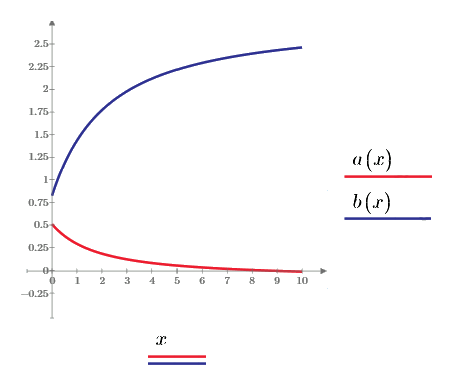
\includegraphics[width=0.8\linewidth]{ab_rab} 	
		\caption{Коэффициенты переноса $a(x)$ и диффузии $b(x)$}
		\label{ris:experimoriginal}
	\end{minipage}
	\hfill
	\begin{minipage}[h]{0.49\linewidth}
		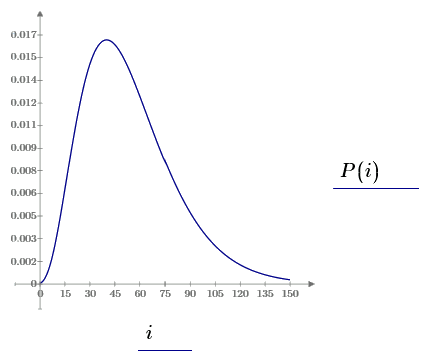
\includegraphics[width=0.8\linewidth]{pb_rab} 
		\caption{Ряд распределения вероятностей количества заявок на орбите}
		\label{ris:experimcoded}
	\end{minipage}
\end{figure}
Данные графики были построены с помощью приложения Mathcad.